\documentclass{article}
\usepackage[utf8]{inputenc}
\usepackage[margin=0.35in]{geometry}


\title{Computer Networks Lab 1}
\author{Shane Cincotta }
\date{March 11, 2020}

\usepackage{natbib}
\usepackage{graphicx}

\begin{document}

\maketitle

\begin{figure}[h!]
\centering
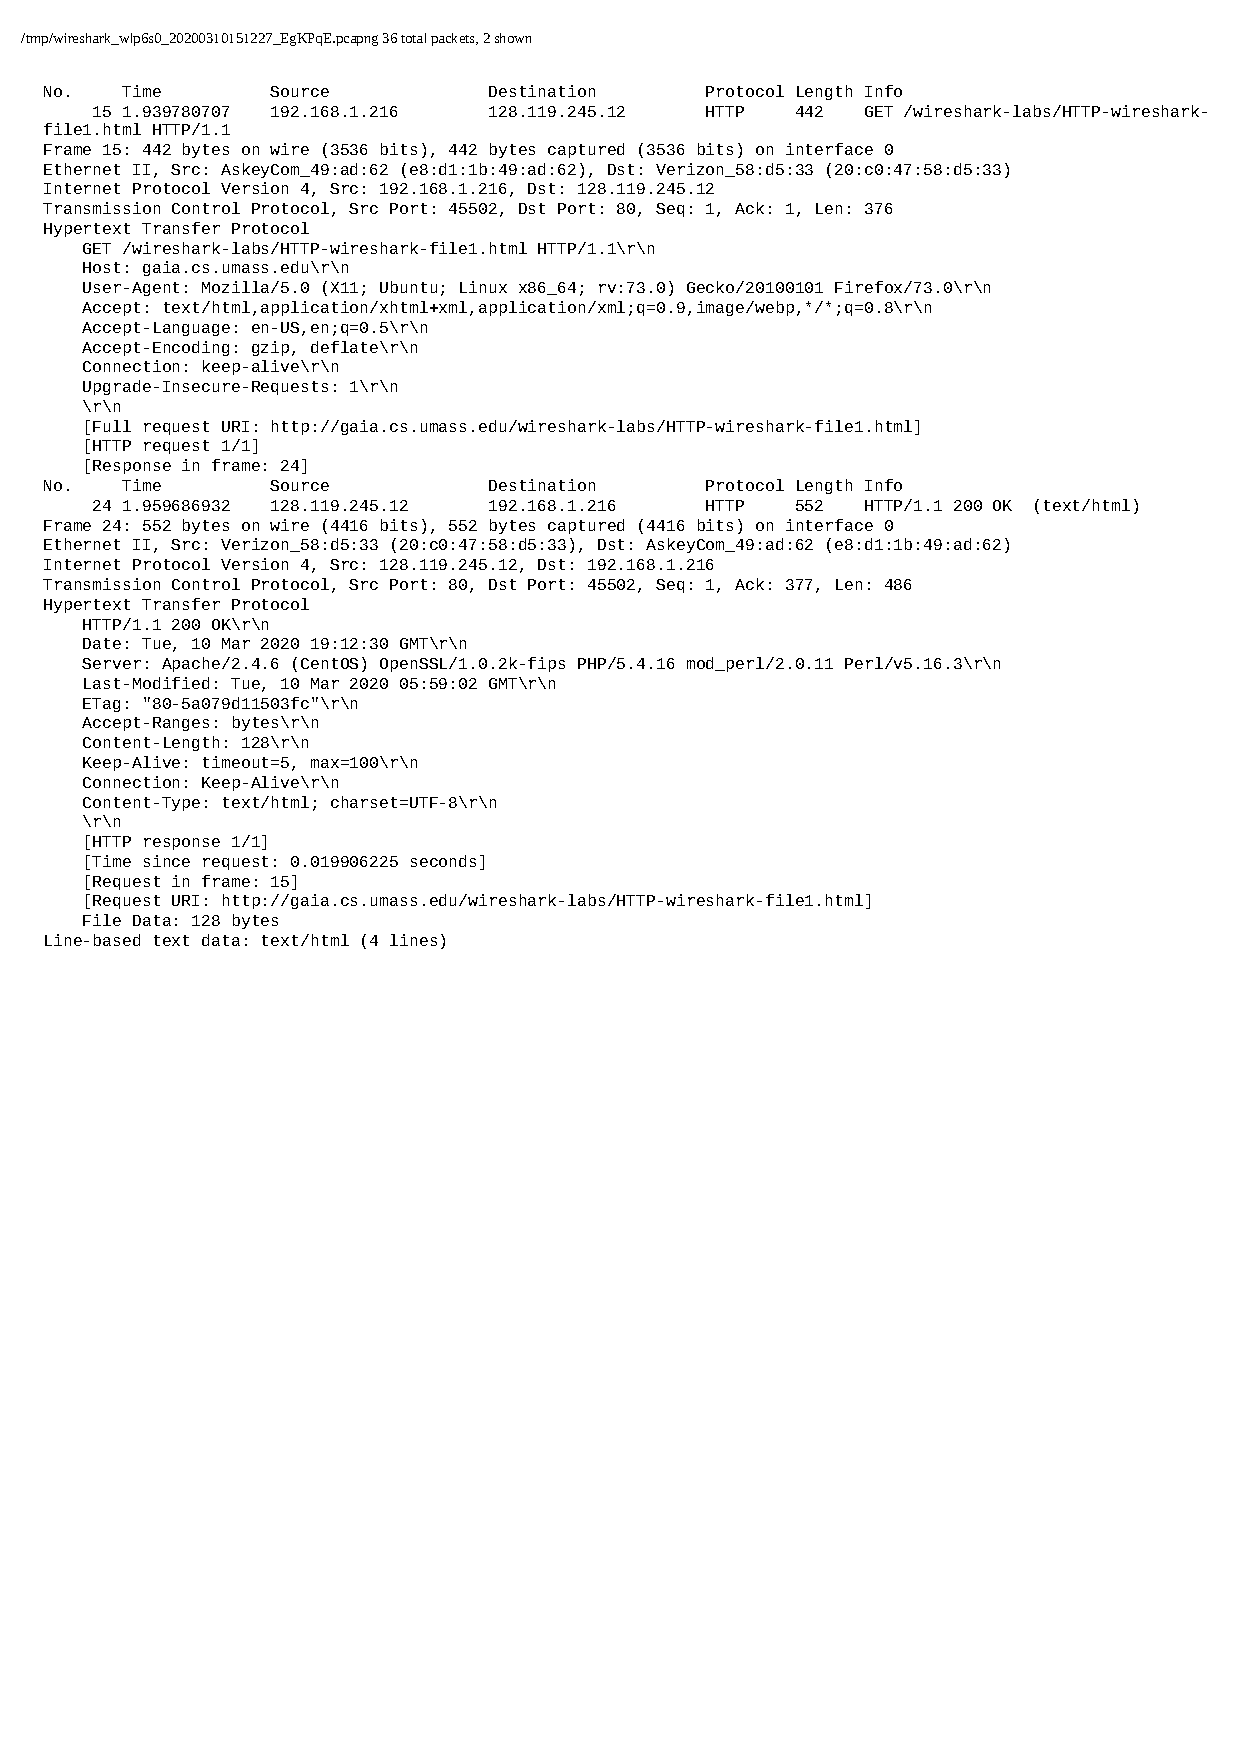
\includegraphics[scale=0.65]{Q1-7Output.pdf}
\caption{}
\end{figure}
\section{Is your browser running HTTP version 1.0 or 1.1? What version of HTTP is the
server running?}
a)  According to figure 1, my browser is running HTTP version 1.1.\\
\newline b)  According to figure 1, the server is running HTTP version 1.1.\\
\section{What languages (if any) does your browser indicate that it can accept to the
server?}
a)  According to figure 1, my browser can accept en-US, en.\\
\section{What is the IP address of your computer? Of the gaia.cs.umass.edu server?}
a)  According to figure 1, the IP address of my computer is 192.168.1.216\\
\newline b)  According to figure 1, the IP address of the server is 128.119.245.12\\
\section{What is the status code returned from the server to your browser?}
a)  According to figure 1, the status code returned is HTTP/1.1 200 OK (text/html)\\
\section{When was the HTML file that you are retrieving last modified at the server?}
a)  According to figure 1, the HTML was Last-Modified: Tue, 10 Mar 2020 05:59:02 GMT\\
\section{How many bytes of content are being returned to your browser?}
a)  According to figure 1, there are 128 bytes of content being returned to my browser.\\
\section{By inspecting the raw data in the packet content window, do you see any headers
within the data that are not displayed in the packet-listing window? If so, name
one.}
a)  No, I don't see any headers that are not displayed in the packet-listing window.
\newline \\
\newline \\
\newline \\
\newline \\
\newline \\
\newline \\
\begin{figure}[h!]
\centering
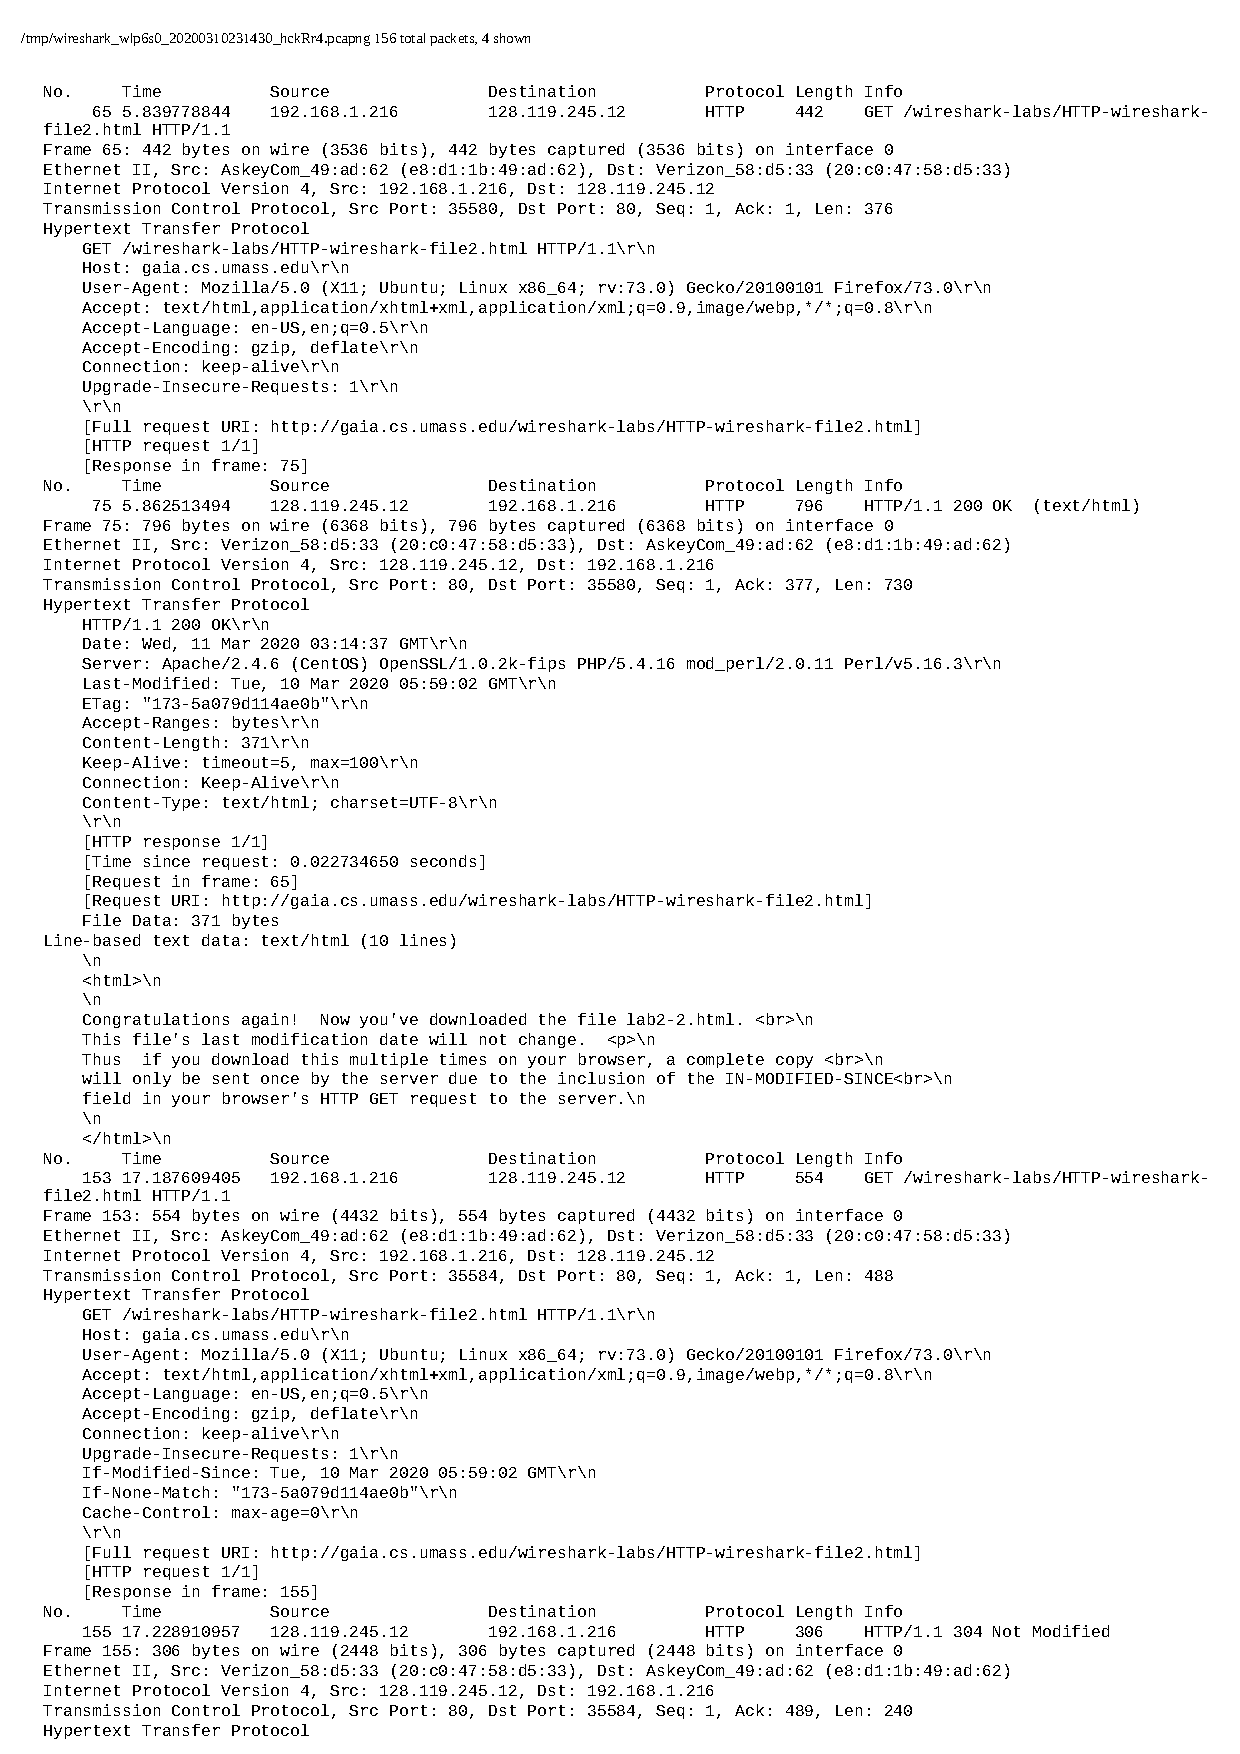
\includegraphics[scale=0.40]{Q8-11Output.pdf}
\caption{}
\end{figure}
\section{Inspect the contents of the first HTTP GET request from your browser to the
server. Do you see an “IF-MODIFIED-SINCE” line in the HTTP GET?}
a)  According to figure 2, I do not see an "IF-MODIFIED-SINCE" line in the HTTP GET.\\
\section{Inspect the contents of the server response. Did the server explicitly return the
contents of the file? How can you tell?}
a)  According to figure 2, yes the server did.  I can tell because I can see the contents of the file in the "Line-based text data" field.\\
\section{Now inspect the contents of the second HTTP GET request from your browser to
the server. Do you see an “IF-MODIFIED-SINCE:” line in the HTTP GET? If
so, what information follows the “IF-MODIFIED-SINCE:” header?}
a)  According to figure 2, yes.  The information that follows is: Tue, 10 Mar 2020 05:59:02 GMT which is the date of the last modification of the file from the previous get request.\\
\section{What is the HTTP status code and phrase returned from the server in response to
this second HTTP GET? Did the server explicitly return the contents of the file?
Explain.}
a)  According to figure 2, the status code and phrase returned from the server is HTTP/1.1 304 Not
Modified. The server didn’t return the contents of the file since the browser loaded it
from its cache.\\
\begin{figure}[h!]
\centering
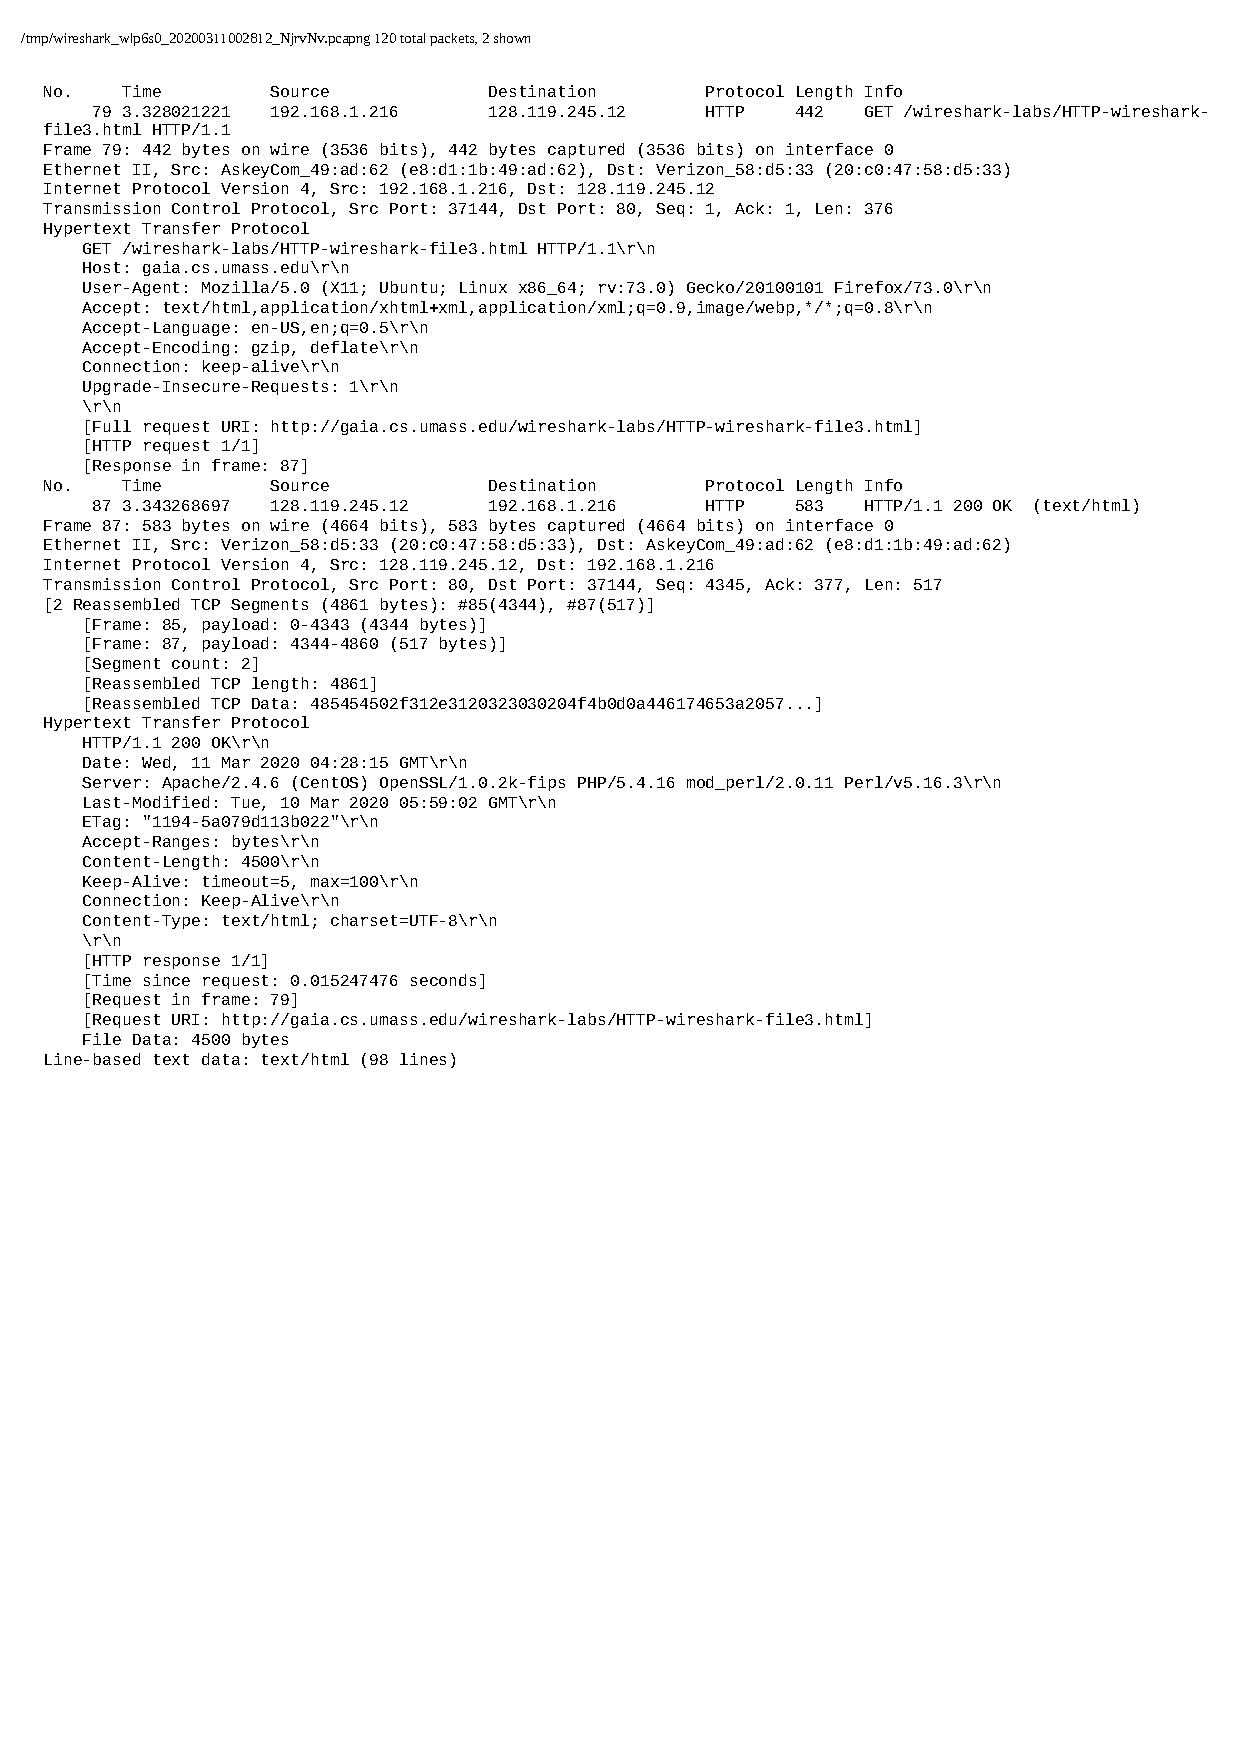
\includegraphics[scale=0.65]{Q12-15Output.pdf}
\caption{}
\end{figure}
\section{How many HTTP GET request messages did your browser send? Which packet
number in the trace contains the GET message for the Bill or Rights?}
a)  According to figure 3, there was 1 HTTP GET requests message that my browser sent.\\
\newline b)  According to figure 3, the packet is number 79 in the trace.\\
\section{Which packet number in the trace contains the status code and phrase associated
with the response to the HTTP GET request?}
a)  According to figure 3, the packet number in the trace which contains the status code and phrase is 87.\\
\section{What is the status code and phrase in the response?}
a)  According to figure 3, the status code is 200 and the phrase in the response is "OK".\\
\section{How many data-containing TCP segments were needed to carry the single HTTP
response and the text of the Bill of Rights?}
a)  According to figure 3, 2 TCP segments were needed to carry the single HTTP response.\\
\begin{figure}[h!]
\centering
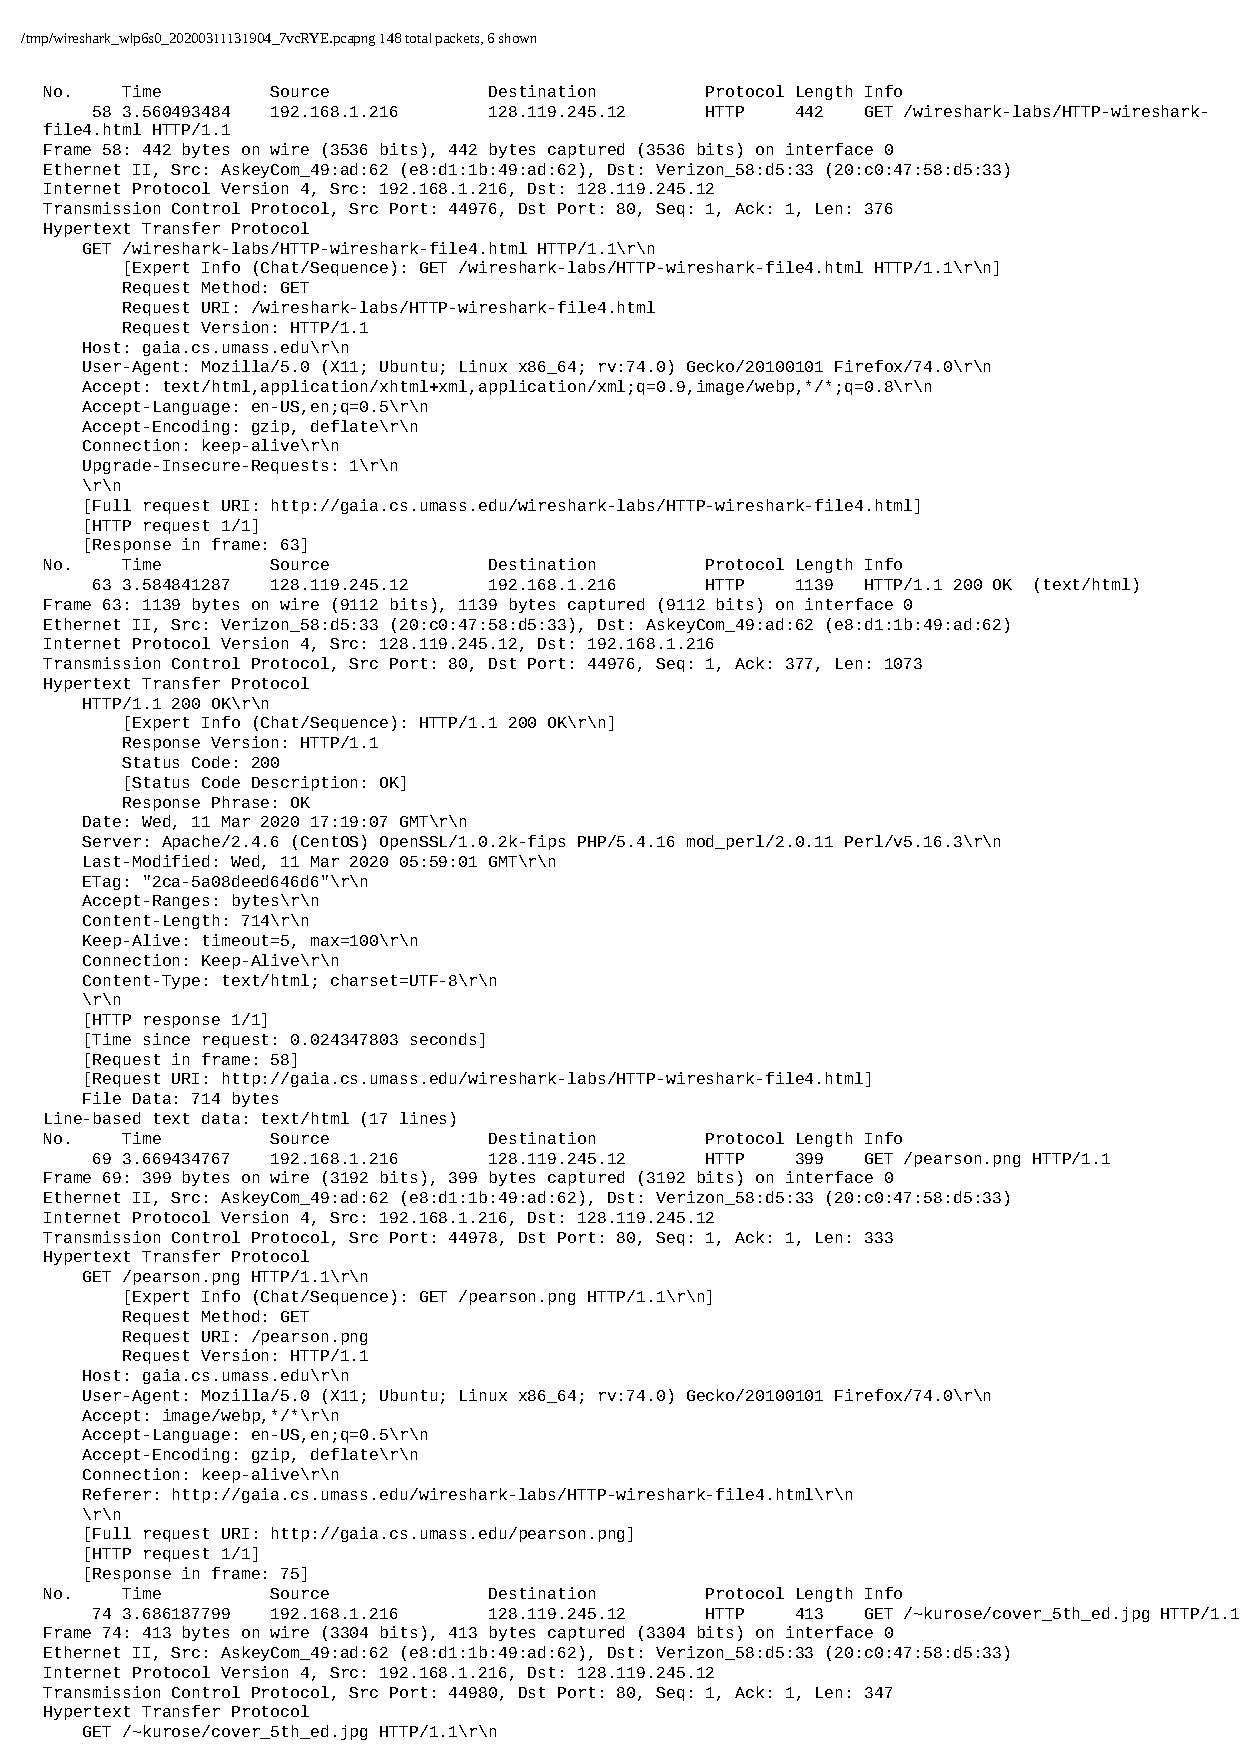
\includegraphics[scale=0.45]{Q16-17Output.pdf}
\caption{}
\end{figure}
\section{How many HTTP GET request messages did your browser send? To which
Internet addresses were these GET requests sent?}
a)  According to figure 4, there were 3 GET messages sent\\
\newline b)  According to figure 4, the get messages were sent to 128.119.245.12\\
\section{Can you tell whether your browser downloaded the two images serially, or
whether they were downloaded from the two web sites in parallel? Explain.}
a)  We can look at the GET messages and determine if the images were sent in serial or parallel.  According to figure 4, the GET messsage for the second image was sent before the first image was received.  Thus the images were sent in parallel.\\
\begin{figure}[h!]
\centering
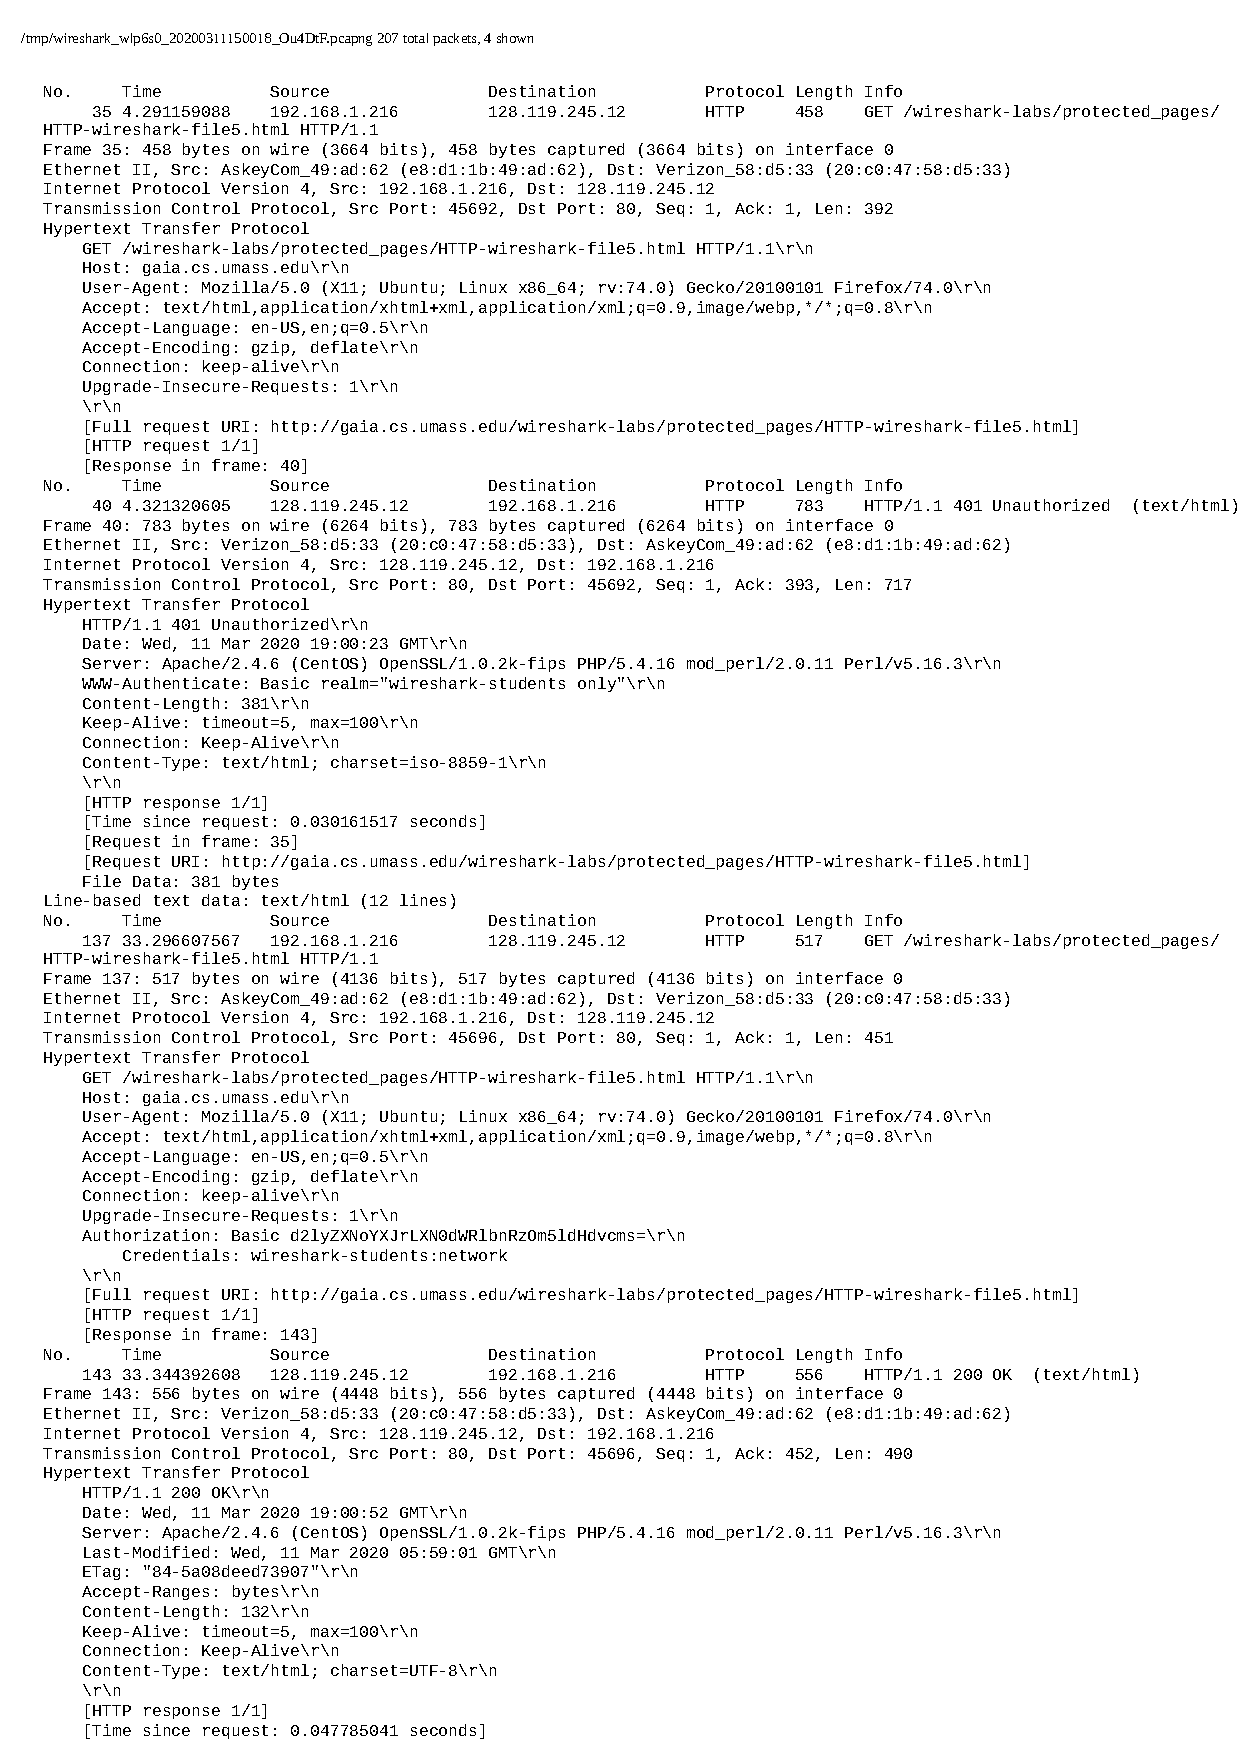
\includegraphics[scale=0.45]{Q18-19Output.pdf}
\caption{}
\end{figure}
\section{What is the server’s response (status code and phrase) in response to the initial
HTTP GET message from your browser?}
a)  According to figure 5, the server's response is 401 Unauthorized.\\
\section{When your browser’s sends the HTTP GET message for the second time, what
new field is included in the HTTP GET message?}
a) According to figure 5, an Authorization field is now added.\\
\end{document}